\documentclass[10pt]{article}
    \usepackage[utf8]{inputenc}
    \usepackage{amsmath}
    \usepackage[margin=0.5in]{geometry}
    \usepackage{graphicx}
    \usepackage{caption}

    \title{Computational Neuroscience \\\ Spike Analysis}
    \author{David Sharp : ds16797 : Candidate 36688}
    \date{March 2019}

    \begin{document}
    \maketitle
    \section{Question One}
    For a Poisson generated spike train of 1000 seconds length with firing rate 35Hz,
    the calculated spike metrics were - for windows of width 10ms, 50ms, and 100ms respectively.
    \subsection{Refractory Period 0ms}
    \textbf{Fano Factors} : \underline{0.65629} (10ms Window), \underline{1.00133} (50ms Window), \underline{1.76023} (100ms Window), 5dp.
    \newline
    \textbf{Coefficient of Variation} :  \underline{1.36530}, 5dp.

    \subsection{Refractory Period 5ms}
    \textbf{Fano Factor} : \underline{0.426047} (10ms Window), \underline{1.00143} (50ms Window), \underline{1.76081} (100ms Window), 5dp.
    \newline
    \textbf{Coefficient of Variation} : \underline{265.09924}, 5dp.

    \section{Question Two}
    For the spike train located in rho.dat,
    the calculated spike metrics were - for windows of width 10ms, 50ms, and 100ms respectively.
    \newline
    \textbf{Fano Factors} : \underline{0.553338} (10ms Window), \underline{2.03108} (50ms Window), \underline{3.73864} (100ms Window), 5dp.
    \newline
    \textbf{Coefficient of Variation} :  \underline{2.00859}, 5dp.

    \section{Question Three}
    \begin{figure}
        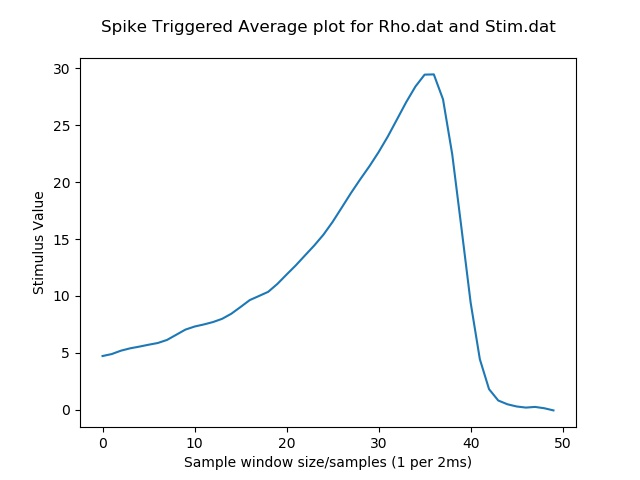
\includegraphics[width=10cm ]{sta.jpg}
        \label{fig:staGraph}
    \end{figure}


\end{document}
